\chapter{phase transitions: criticality, universality, and scaling}
\begin{itemize}
	\item 热力学系统可以分为两类: noninteracting \& interacting.
	
	\item noninteracting 的系统包括: the specific heat of gases (section \ref{1.2} and \ref{6.4}); the specific heat of solids (section \ref{7.4}); chemical equilibrium in an ideal gas or a dilute solution (section \ref{6.5}); condensation of an ideal Bose gas (section \ref{7.1} and \ref{7.2}); spectral distribution of the blackbody radiation (section \ref{7.3}); the free electron theory of metals (section \ref{8.3}); the phenomenon of paramagnetism (section \ref{3.7} and \ref{8.2}).
	\begin{itemize}
		\item 除了 Bose--Einstein condensation 之外, 所有这些系统的 thermodynamic functions 都是光滑的.
	\end{itemize}
	
	\item interacting 的系统包括: the condensation of gases; the melting of solids; the coexistence of phases (especially near a critical point); mixtures and solutions (包括 the onset of phase separation); ferromagnetism and antiferromagnetism; the order--disorder transitions in alloys; the superfluid transition from liquid He I to liquid He II; transition from a normal to a superconducting material.
	\begin{itemize}
		\item interacting 的系统, 经常会遇到 thermodynamic functions 具有 analytic discontinuities or singularities 的情况, 相应地, 会遇到各种 phase transitions.
	\end{itemize}
\end{itemize}

\section{general remarks on the problem of condensation}
\begin{itemize}
	\item 对任何热力学系统, 都有
	\begin{equation}
		\Big( \frac{\partial P'}{\partial v} \Big)_{V, T} = - \frac{k_B T}{v^2} \frac{\braket{N}}{\braket{(\Delta N)^2}} \leq 0,
	\end{equation}
	其中 $P'$ 定义为
	\begin{equation}
		P' := \frac{k_B T}{V} \ln Z_\text{GC} \equiv - \frac{\Phi_\text{G}}{V},
	\end{equation}
	对于 homogeneous system (注意 multiphase systems 也可以是 homogeneous, 但要忽略表面效应) 有 $P' = P$.
	
	\begin{tcolorbox}[title=calculation:]
		注意到
		\begin{equation}
			- \frac{V}{N^2} \Big( \frac{\partial P'}{\partial v} \Big)_{T, V} = \Big( \frac{\partial P'}{\partial N} \Big)_{T, V} = - \frac{1}{V} \Big( \frac{\partial \Phi_\text{G}}{\partial N} \Big)_{T, V},
		\end{equation}
		且
		\begin{equation}
			\Big( \frac{\partial \Phi_\text{G}}{\partial N} \Big)_{T, V} = - N \Big( \frac{\partial \mu}{\partial N} \Big)_{T, V} = - \frac{N}{\big( \frac{\partial N}{\partial \mu} \big)_{T, V}} = - \frac{N}{\beta \braket{(\Delta N)^2}},
		\end{equation}
		最后一个等号用到了 \eqref{4.4.1}.
	\end{tcolorbox}
	
	\item 注意到, 在某些区间, $\braket{(\Delta N)^2} \sim O(N^2)$, 此时
	\begin{equation}
		\Big( \frac{\partial P'}{\partial v} \Big)_{V, T} \sim O(N^{- 1}) \simeq 0.
	\end{equation}
\end{itemize}

\section{condensation of a van der Waals gas}
\begin{itemize}
	\item van der Waals gas 满足 equation of state 为
	\begin{equation}
		P = \frac{k_B T}{v - b} - \frac{a}{v^2} \quad \text{or} \quad P_r = \frac{8 T_r}{3 v_r - 1} - \frac{3}{v_r^2},
	\end{equation}
	其中 $P_r = \frac{P}{P_c}, v_r = \frac{v}{v_c}, T_r = \frac{T}{T_c}$, 且
	\begin{equation}
		P_c = \frac{a}{27 b^2}, \quad v_c = 3 b, \quad T_c = \frac{8 a}{27 b k_B}. \upsilon v
	\end{equation}
	
	\item van der Waals gas 的 isotherms 如下图所示:
	
	\begin{figure}[H]
		\centering
		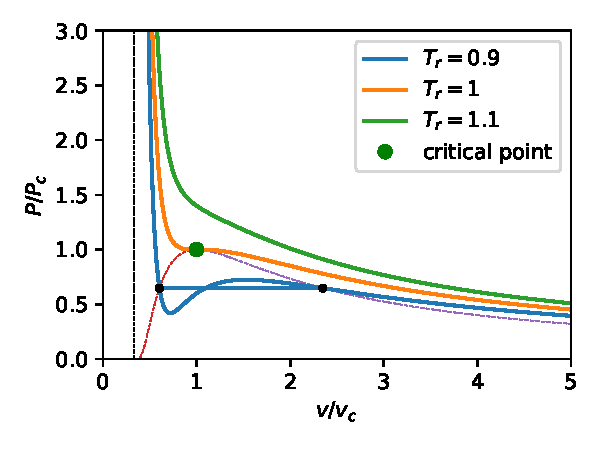
\includegraphics[scale=0.8]{figures/isotherms of the van der Waals gas.pdf}
		\caption{isotherms of the van der Waals gas.}
	\end{figure}
	
	\begin{itemize}
		\item 具体的计算细节可以参考 Wikipedia page: \href{https://en.wikipedia.org/wiki/Van_der_Waals_equation#Saturation}{van der Waals equation: saturation}.
	\end{itemize}
	
	\item 
\end{itemize}
